\section{Planar Objects}
The form factor of very anisotropic particles with local planar
geometry can be shown to factorize (see, e.g., Porod, 1948) into a
cross section form factor $P_\text{cs}(Q)$ for the shorter
dimensions and a shape factor $P'(Q)$ for the larger dimension:
\begin{align}
P_\text{planar}(Q) = P'(Q) P_\text{cs}(Q)
\end{align}
The shape form factor $P'(Q)$ can be that of an infinitely thin
spherical shell, elliptical shell, cylindrical shell, or disk. In
the following the shape form factor is assumed to the one of an
infinitely thin disk:
\begin{align}
P'(Q,R)=\frac{2\pi^2R^4}{(QR)^2}
\left(1-\frac{\text{J}_1(2QR)}{QR}\right)
\end{align}
\\

\clearpage
\subsection{homogeneousXS}
\label{sect:homogeneousXS}
\hspace{1pt} \\
\begin{figure}[htb]
\begin{center}
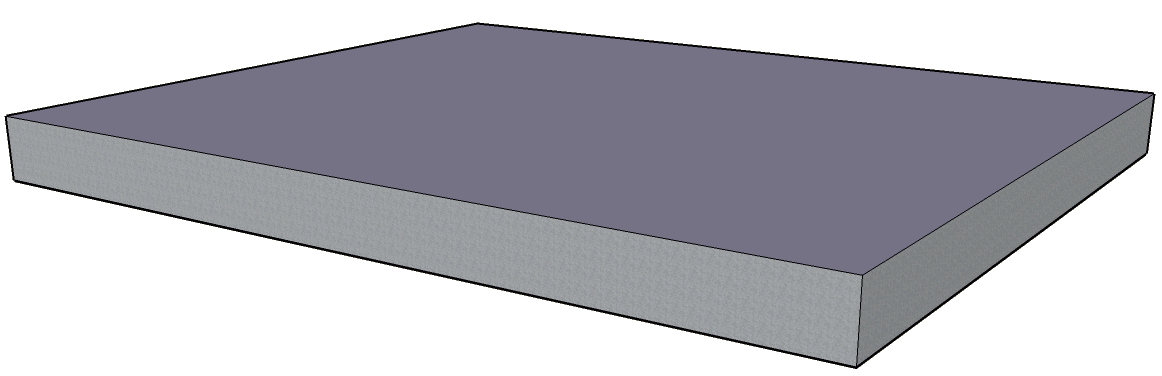
\includegraphics[width=0.6\textwidth,height=0.4\textwidth]{planarHomo.png}
\end{center}
\caption{Planar object with homogeneous cross-section.}
\label{fig:planarHomo}
\end{figure}

\begin{align}
P_\text{cs}(Q,\eta,L) = \left( \eta L\frac{\sin(QL/2)}{QL/2}\right)^2
\end{align}
%%%%%%%%%%%%%%%%%%%%%%%%%%%%%%%%%%%%%%%%%%%%%%%%%%%%%%%%%%%%%%%%%%%%%

\clearpage
\subsection{TwoInfinitelyThinPlates}
\label{sect:TwoInfinitelyThinPlates}
\hspace{1pt} \\
\begin{figure}[htb]
\begin{center}
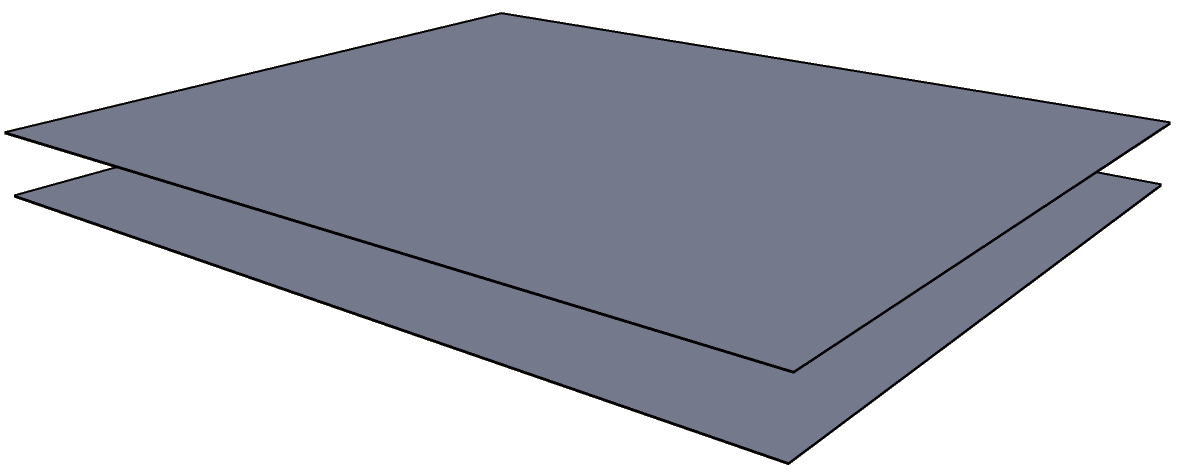
\includegraphics[width=0.6\textwidth,height=0.4\textwidth]{planar2thin.png}
\end{center}
\caption{planar2thin.}
\label{fig:planar2thin}
\end{figure}
\begin{align}
P_\text{cs}(Q,\eta,L) = \eta^2 \cos^2(QL/2)
\end{align}


%%%%%%%%%%%%%%%%%%%%%%%%%%%%%%%%%%%%%%%%%%%%%%%%%%%%%%%%%%%%%%%%%%%%%
\clearpage
\subsection{LayeredCentroSymmetricXS}
\label{sect:LayeredCentroSymmetricXS}
~\\

\begin{figure}[htb]
\begin{center}
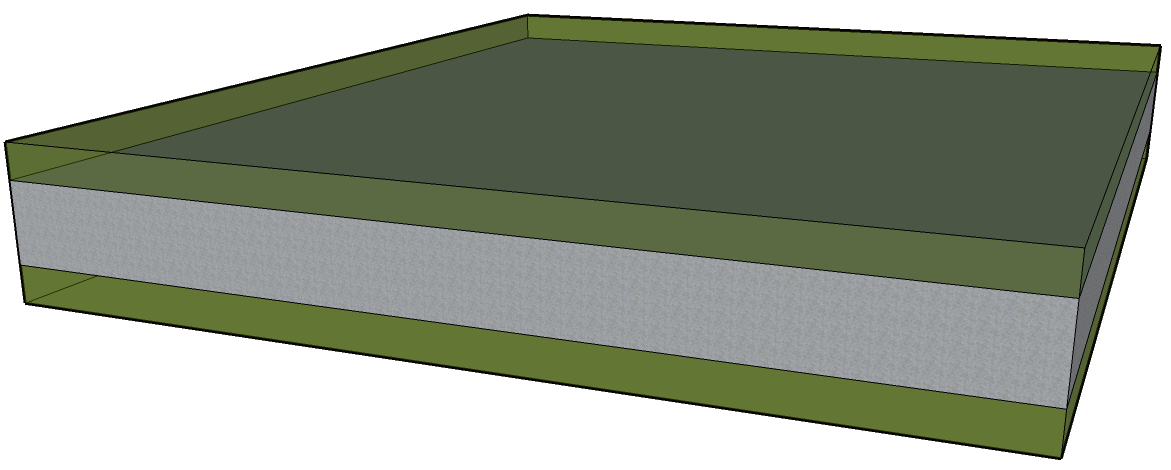
\includegraphics[width=0.6\textwidth,height=0.4\textwidth]{planar2centrosymm.png}
\end{center}
\caption{planar2centrosymHomo.}
\label{fig:planar2centrosymm}
\end{figure}
A layered centro symmetric cross-section structure with outer
thickness $L_\text{out}$ and a core of thickness $L_c$, where the
core and the outer part have the scattering lengths density
$\eta_\text{out}$ and $\eta_c$, respectively, has
\begin{align}
P_\text{cs}(Q,\eta_\text{out},L_\text{out},\eta_c,L_c)
= \Biggl( & \frac{\eta_\text{out}L_\text{out}\sin\left(\frac{QL_\text{out}}{2}\right)}{QL_\text{out}/2} \\
&-  \frac{(\eta_\text{out}-\eta_c)L_c\sin\left(\frac{QL_c}{2}\right)}{QL_c/2}\Biggr)^2 \nonumber
\end{align}

%%%%%%%%%%%%%%%%%%%%%%%%%%%%%%%%%%%%%%%%%%%%%%%%%%%%%%%%%%%%%%%%%%%%%%%%%

\clearpage
\subsection{BiLayerGauss}
\label{sect:BiLayerGauss}
~\\
\begin{figure}[htb]
\begin{center}
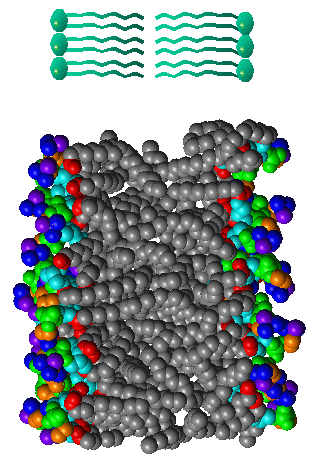
\includegraphics[width=0.4\textwidth,height=0.5\textwidth]{BiLayers.png}
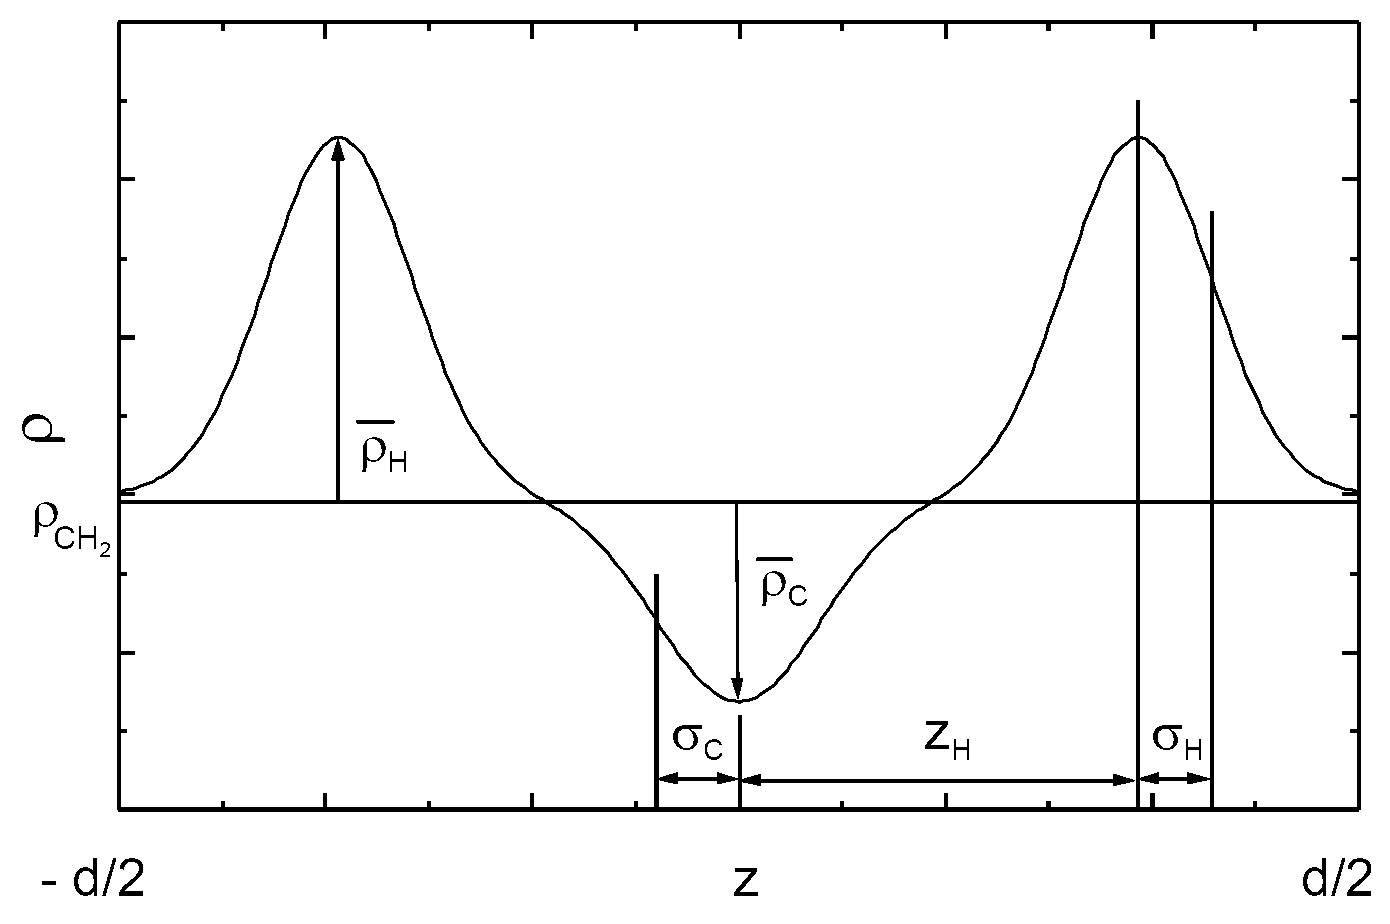
\includegraphics[width=0.5\textwidth,height=0.4\textwidth]{bilayerprofile.png}
\end{center}
\caption{bilayerprof.}
\label{fig:bilayerprof}
\end{figure}

\begin{align}
   u_\text{out}  &= Q\sigma_\text{out} \\
   u_\text{core} &= Q\sigma_\text{core} \\
   F_\text{out}  &= \sqrt{2\pi}\sigma_\text{out}  b_\text{out}  \exp(-u_\text{out}^2/2) \cos(Qt/2) \\
   F_\text{core} &= \sqrt{2\pi}\sigma_\text{core} b_\text{core} \exp(-u_\text{core}^2/2)  \\
   P_\text{cs}   &=(F_\text{core}+2 F_\text{out})^2
\end{align}
